\chapter*{Transfer function measurement software}\label{appendix:transfer_function}
In this appendix the transfer function software will be briefly explained. The gold of this software is to be able to compute the impulse response of a \gls{dut} using the logarithmic swept sine method and then compute the transfer function from the impulse response. To be able to send out a logarithmic swept sine and measure it, a full duplex soundcard have to be chosen and used as the measuring soundcard. To be able to reproduce all measurement and compare other measurement, the soundcard will not be changed doing the project work.

\section*{Materials and setup}
To measure transfer function of a \gls{dut}, the following materials are used:
\begin{itemize}
\item RME FIREFACE ucx (Soundcard)
\begin{itemize}[noitemsep]
\item AAU-number: 108230
\item Serial number: 23811948
\end{itemize}
\item MATLAB (PC - software)
\item \gls{usb} A to \gls{usb} B cable
\end{itemize}



\begin{figure}[H]
\centering
\begin{picture}(0,0)%
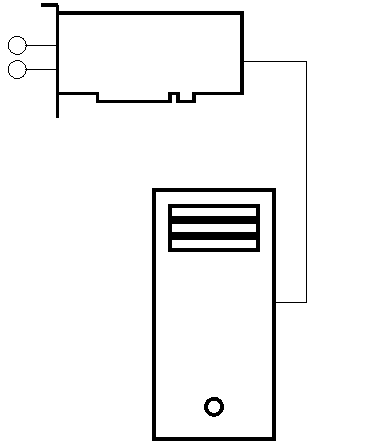
\includegraphics{transfer_function.pdf}%
\end{picture}%
\setlength{\unitlength}{2818sp}%
%
\begingroup\makeatletter\ifx\SetFigFont\undefined%
\gdef\SetFigFont#1#2#3#4#5{%
  \reset@font\fontsize{#1}{#2pt}%
  \fontfamily{#3}\fontseries{#4}\fontshape{#5}%
  \selectfont}%
\fi\endgroup%
\begin{picture}(4090,4926)(8176,-7474)
\put(8191,-3661){Out}%
\put(9271,-3211){Sound Card}%
\put(9971,-6361){Computer}%
\put(11836,-4696){USB}%
\put(8281,-2806){In}%
\end{picture}%
\caption{Setup for measuring transfer function}
		\label{fig:appendix:transfer_function}
\end{figure}

\section*{Transfer function software}
The software is made as a function where one can get the impulse response and transfer function and there time and frequency x-axis vector respectively. The function name is:

\includeCode{IRmeas_fft.m}{matlab}{1}{1}{The turntable control function}{code:ET250_3D}{./code/sine_swept/}

To get output from this function, the following variable have to be initialised.



 \begin{table}[H]
\centering
\caption{Function command}
\label{my-label}
\begin{tabular}{lll}
 & $ts$ & Which is the length of the logarithmic swept sine  \\
 & $tw$ & Which is a silence there can be added to the logarithmic swept sine in end   \\
 & $flower$ & Which is the lower frequency border for logarithmic swept sine   \\
 & $fupper$ & Which is the upper frequency border for logarithmic swept sine  \\
 & $playgain$ & Which is the gain for logarithmic swept sine playback   \\
 & $player$  & Which is the initializing I-O via the soundcard
\end{tabular}
\end{table}



\section*{The MATLAB function}
\includeCode{IRmeas_fft.m}{matlab}{1}{82}{The turntable control function}{code:ET250_3D}{./code/sine_swept/}

